% -*- coding: UTF-8 -*-
\documentclass{article}
\usepackage{amsmath}
\usepackage{tikz}


\begin{document}
\begin{tikzpicture}

  \draw[->] (-1.5,0) -- (7,0);
  \draw[->] (0,-2) -- (0,3);
  \node[below] at (7,0) {$t$};
  \node[left] at (0,3) {$d$};

  \node[below] at ({rad(180)},0) {$\pi$};
  \draw (0,2) -- (0.125,2);
  \node[left] at (0,2) {$2$};
  \node[below left] at (0,0) {$O$};

  \draw[thick, domain=0:rad(360)] plot (\x, {2*abs(sin(\x r))});

  \node at (2.75,-2) {(A)};

\end{tikzpicture}

\begin{tikzpicture}

%  \begin{scope}[xshift=9cm]

  \draw[->] (-1.5,0) -- (7,0);
  \draw[->] (0,-2) -- (0,3);
  \node[below] at (7,0) {$t$};
  \node[left] at (0,3) {$d$};

  \node[below] at ({rad(135)},0) {$\tfrac{3\pi}4$};
  \draw (0,2) -- (0.125,2);
  \node[left] at (0,2) {$2$};
  \draw (0,1.414) -- (0.125,1.414);
  \node[left] at (0,1.414) {$\sqrt2$};
  \node[below left] at (0,0) {$O$};

  \draw[thick, domain=0:rad(135)] plot (\x, {sqrt(2)*abs(sin(\x r)+cos(\x r))});
  \draw[thick, domain=rad(135):rad(315)] plot (\x, {sqrt(2)*abs(sin(\x r)+cos(\x r))});

  \node at (2.75,-2) {(B)};

 % \end{scope}


\end{tikzpicture}

\begin{tikzpicture}

  \begin{scope}[xshift=18cm]

  \draw[->] (-1.5,0) -- (7,0);
  \draw[->] (0,-2) -- (0,3);
  \node[below] at (7,0) {$t$};
  \node[left] at (0,3) {$d$};

  \node[below] at ({rad(45)},0) {$\tfrac{\pi}4$};
  \draw (0,2) -- (0.125,2);
  \node[left] at (0,2) {$2$};
  \draw (0,1.414) -- (0.125,1.414);
  \node[left] at (0,1.414) {$\sqrt2$};
  \node[below left] at (0,0) {$O$};

  \draw[thick, domain=0:rad(360)] plot (\x, {sqrt(2)*abs(sin(\x r)-cos(\x r))});

  \node at (2.75,-2) {(C)};

  \end{scope}


\end{tikzpicture}

\begin{tikzpicture}

  \begin{scope}[xshift=27cm]

  \draw[->] (-1.5,0) -- (7,0);
  \draw[->] (0,-2) -- (0,3);
  \node[below] at (7,0) {$t$};
  \node[left] at (0,3) {$d$};

  \node[below] at ({rad(45)},0) {$\tfrac{\pi}4$};
  \draw (0,2) -- (0.125,2);
  \node[left] at (0,2) {$2$};
  \node[below left] at (0,0) {$O$};

  \draw[thick, domain=0:rad(90)] plot (\x, {cos(4*\x r)+1});
  \draw[thick, domain=rad(90):rad(180)] plot (\x, {cos(4*\x r)+1});
  \draw[thick, domain=rad(180):rad(270)] plot (\x, {cos(4*\x r)+1});

  \node at (2.75,-2) {(D)};

  \end{scope}


\end{tikzpicture}

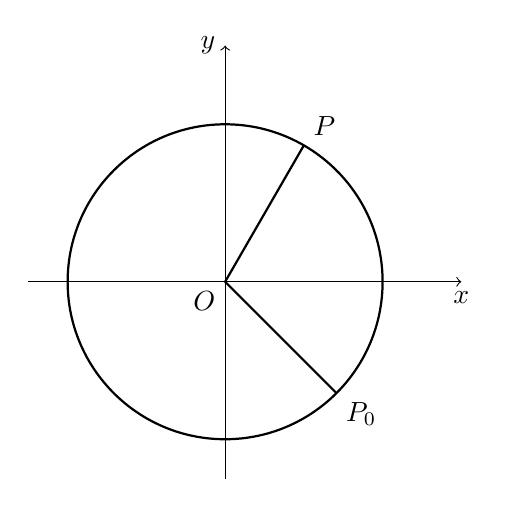
\begin{tikzpicture}

  \begin{scope}[xshift=37cm]

  \draw[->] (-2.5,0) -- (3,0);
  \draw[->] (0,-2.5) -- (0,3);
  \node[below] at (3,0) {$x$};
  \node[left] at (0,3) {$y$};
  \node[below left] at (0,0) {$O$};

  \coordinate[label=60:$P$] (p) at (60:2);
  \coordinate[label=-45:$P_0$] (p0) at (-45:2);


  \draw[thick] (p) -- (0,0) -- (p0) (0,0) circle (2);

  \end{scope}

\end{tikzpicture}
\end{document}
